\chapter{Evaluation Protocol}
\label{chap:eval}

\section{Dice Similarity Coefficient}

The primary metric is the Dice Similarity Coefficient (DSC), also called the F1-score in the
volumetric segmentation context. For organ class~$c$ in volume~$v$, let $P_{v,c}$ denote the
set of predicted voxels and $G_{v,c}$ the set of ground-truth voxels. Dice is defined as:

\begin{equation}
  \mathrm{DSC}(P_{v,c},\, G_{v,c}) = \frac{2\,|P_{v,c} \cap G_{v,c}|}{|P_{v,c}| + |G_{v,c}|}
  \label{eq:dice}
\end{equation}

The mean Dice reported throughout this report averages over all organs present in each
validation volume and then over all validation volumes.

\section{95th-Percentile Hausdorff Distance}

The 95th-percentile Hausdorff Distance (HD95) measures boundary accuracy. For organ~$c$ in
volume~$v$, let $S_P$ and $S_G$ be the sets of surface voxels of the prediction and
ground-truth, respectively. The directed Hausdorff distance from $S_P$ to $S_G$ is
$\sup_{p \in S_P} \inf_{g \in S_G} d(p, g)$. The symmetric HD95 uses the 95th percentile of
all pairwise surface distances in both directions:

\begin{equation}
  \mathrm{HD95} = \operatorname{percentile}_{95}\!\left(
    \left\{d(p, S_G)\right\}_{p \in S_P} \cup
    \left\{d(g, S_P)\right\}_{g \in S_G}
  \right)
\end{equation}

By excluding the worst 5\% of surface errors, HD95 is robust to small, isolated prediction
failures that would inflate the standard Hausdorff Distance to extreme values. HD95 values
are reported in both pixels and millimetres; the millimetre conversion uses the per-volume
voxel spacing stored in the NIfTI header.

\section{Test-Time Augmentation}

Test-Time Augmentation (TTA) improves segmentation consistency at zero training cost by
ensembling predictions from multiple views of the same input. The TTA strategy used in this
project applies four spatial transforms to each test slice: the original orientation, horizontal
flip, vertical flip, and both flips simultaneously. The model produces a 14-class softmax
probability map for each transformed version; the four maps are averaged after flipping back to
the original orientation, and the argmax of the averaged map gives the final prediction.

Figure~\ref{fig:tta} illustrates the four-way ensemble.

\begin{figure}[h!]
\centering
\begin{minipage}{0.85\textwidth}
  \centering
  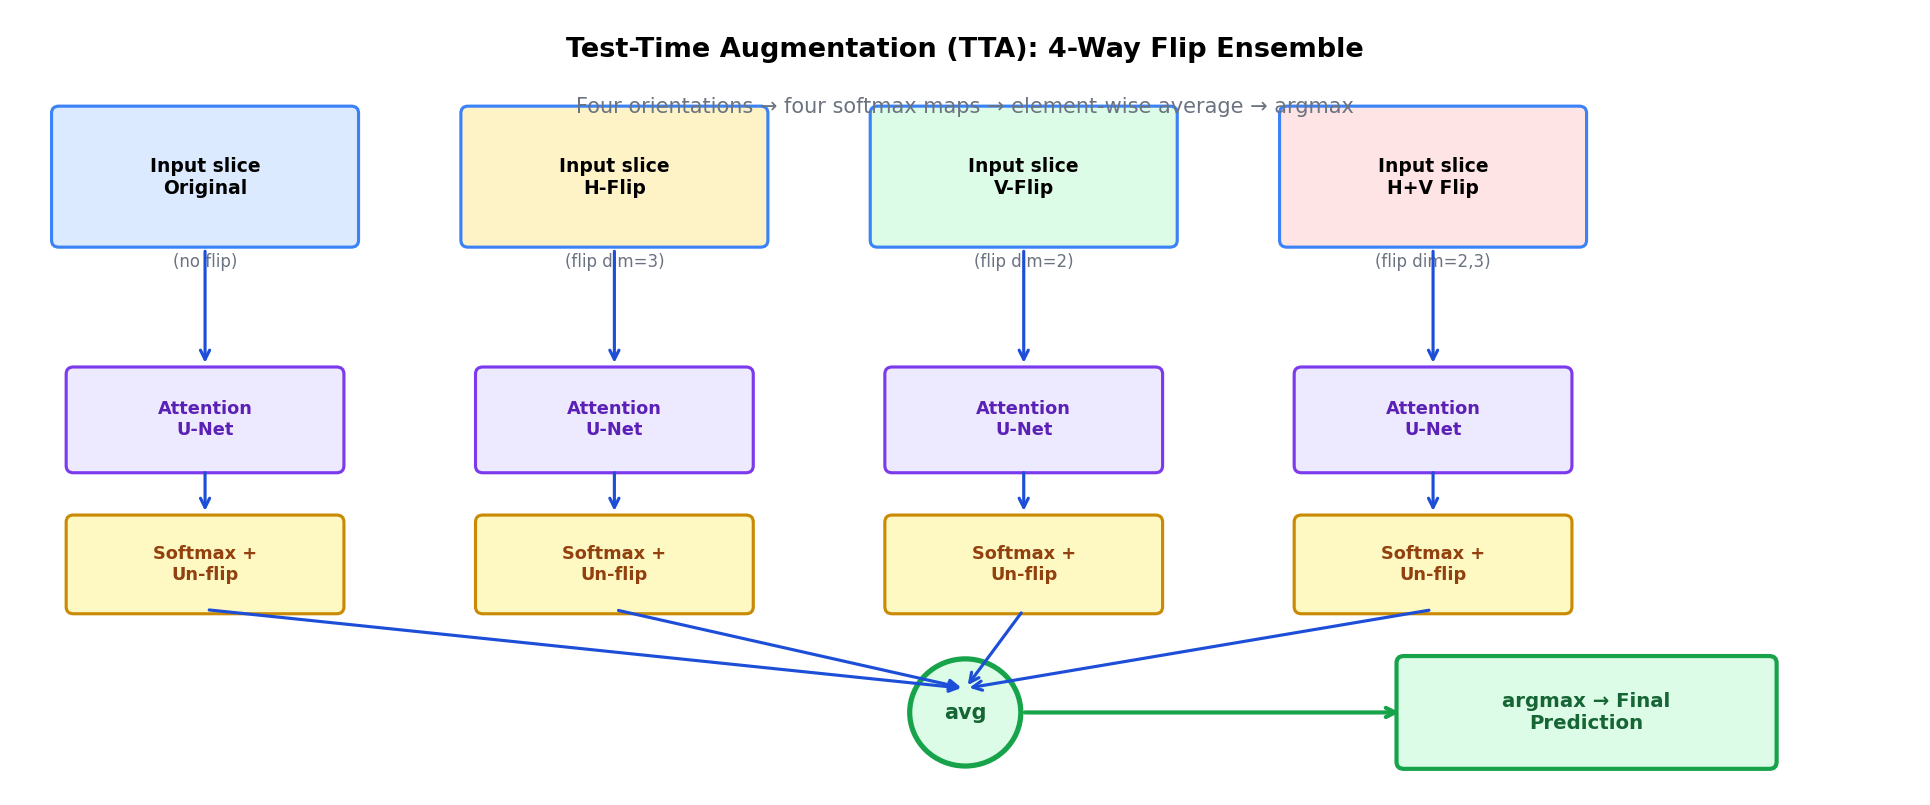
\includegraphics[width=\textwidth]{figures/fig_tta_diagram}
  \caption{Four-way TTA ensemble. Each input slice is transformed into four orientations
  (original, H-flip, V-flip, HV-flip). The model produces a softmax probability map for
  each; predictions are flipped back and averaged. The argmax of the average map is the final
  segmentation.}
  \label{fig:tta}
\end{minipage}
\end{figure}

\FloatBarrier

TTA adds a factor of $4\times$ inference time per slice. For a validation volume with
${\sim}94$ slices this is still under one second on a T4 GPU, making TTA practical even at
deployment time.

\section{Per-Volume Evaluation Protocol}

\subsection{Why Per-Volume, Not Per-Slice?}

An early version of the evaluation code computed Dice per axial slice and averaged across all
slices. This inflated scores significantly. The root cause is empty-slice pairs: in CT volumes,
many slices contain no voxels for a given organ (e.g., the pancreas is absent from the top
third of the abdomen). When both prediction and ground-truth for a class are all-zero on a
slice, the Dice numerator and denominator both evaluate to $\epsilon / (0 + 0 + \epsilon) = 1.0$
under a na\"\i{}ve implementation with a smoothing term. Averaging thousands of such trivial
"perfect" matches over a volume gives a misleadingly high score.

The corrected protocol stacks all predicted slices of a validation volume into a 3D array,
stacks the corresponding ground-truth masks, and computes Dice and HD95 once per organ per
volume on the 3D arrays. For organs with no voxels in ground-truth \emph{and} no voxels in the
prediction, the score is recorded as \texttt{NaN} and excluded from the mean (using
\texttt{numpy.nanmean}). This matches the FLARE22 challenge evaluation script exactly.

\subsection{Implementation}

\begin{verbatim}
for vol_id in val_volume_ids:
    pred_3d = np.zeros((NUM_CLASSES, D, H, W))  # D slices per volume
    gt_3d   = np.zeros((D, H, W))
    for s, slice_idx in enumerate(vol_slices[vol_id]):
        pred_3d[:, s] = model_predict(slice_idx)  # raw softmax probabilities
        gt_3d[s]      = ground_truth[slice_idx]

    for c in range(1, NUM_CLASSES):               # skip background
        pred_c = (pred_3d.argmax(0) == c)
        gt_c   = (gt_3d == c)
        if pred_c.sum() == 0 and gt_c.sum() == 0:
            dice_scores[vol_id][c] = np.nan       # empty -> exclude
        else:
            dice_scores[vol_id][c] = dice_volume(pred_c, gt_c)
\end{verbatim}

All numerical results in Chapter~\ref{chap:results} and Chapter~\ref{chap:ablation} were
computed under this corrected per-volume protocol.
